\documentclass[11pt,a4paper]{article}

\usepackage[T1]{fontenc}
\usepackage[utf8]{inputenc}
\usepackage{lmodern}
\usepackage[margin=2.05cm]{geometry}
\usepackage{amsmath,amssymb}
\usepackage{graphicx}
\usepackage{booktabs}
\usepackage{array}
\usepackage{xcolor}
\usepackage{microtype}
\usepackage[font=small,labelfont=bf]{caption}
\usepackage{subcaption}
\usepackage[numbers,sort&compress]{natbib}
\usepackage[hidelinks]{hyperref}
\usepackage{siunitx}
\sisetup{detect-all}

\setlength{\parskip}{0.35em}
\setlength{\parindent}{0pt}
\renewcommand{\arraystretch}{1.08}
\renewcommand{\topfraction}{0.92}
\renewcommand{\bottomfraction}{0.8}
\renewcommand{\textfraction}{0.08}
\renewcommand{\floatpagefraction}{0.75}

\title{\textbf{Prism on a Laptop:}\\[0.25em]
\large Streaming Inference of a 105B FP8 Mixture-of-Experts Decision Model\\[0.25em]
\large and a Study of Expert Pruning}
\author{Pranav Krishnakumar}
\date{November 2026}

\begin{document}
\maketitle

\begin{abstract}
Prism is a 105B-parameter mixture-of-experts decision model that scores every option of a typed question in one forward pass. We show that it runs correctly on a laptop with an Intel Arc 140V integrated GPU, and that keeping 32 of its 128 routed experts preserves some tasks but not others. A streaming engine reads one decoder layer at a time from an NVMe SSD and runs the 106.2\,GB FP8 model at 32 tokens per second at batch size 64. It matches an FP32 reference, reproduces the model card's choices, and agrees with the hosted API on 93\% of 1,200 questions. The pruned model keeps 78\% of the full model's decisions overall. NLI, sentiment and intent routing stay above 90\%, while knowledge multiple choice falls to 41\% and Hindi, Bengali and Telugu fall below 65\%. The calibration domain matters more than the ranking rule.
\end{abstract}

\section{Introduction}

A decision model answers a question whose options are fixed in advance. It returns one probability per option in a single forward pass and never generates text \citep{sarvam2026prism}. Prism is such a model, built on the 105B-parameter Sarvam mixture-of-experts backbone. Its FP8 weights occupy 106.2\,GB and the model card asks for a GPU with about 120\,GB of memory, while the laptop used here has 16\,GB of shared graphics memory and 32\,GB of RAM. The obstacle is memory, not arithmetic, so the weights must be streamed from disk. Offloading systems for generative inference do this, but they pay the read cost again for every generated token \citep{aminabadi2022deepspeed,sheng2023flexgen,song2024powerinfer}. A decision model has no decode loop, so each layer is read once per batch and batch size controls how far the read is amortised.

Correctness is a separate problem. Prism uses a nonstandard attention mask, multi-head latent attention, a sigmoid-routed mixture of experts and FP8 weights with per-row scales \citep{micikevicius2022fp8}. The integrated GPU has no FP8 matrix multiply, so the engine dequantises just in time and emulates FP8 activations in BF16. We compare the engine with an independent FP32 CPU reference layer by layer, and the full model with the hosted API on 1,200 test questions.

The second question is how much of the model is needed. We rank experts by router statistics from a calibration set, rewrite the router and expert tensors, and measure the pruned model against the full model while varying the number of experts, the ranking rule, the calibration domain and the number of decoder layers. Table~\ref{tab:summary} gives the main results.

The report makes three contributions:
\begin{itemize}
\item A streaming engine that runs the full 106.2\,GB model on a laptop integrated GPU, with layer prefetch, lookup-table dequantisation, the Prism attention mask and a CPU decision head.
\item A verification against an FP32 reference and the hosted API, including an account of a gap to the model card example.
\item A controlled expert-pruning study over 1,200 test questions in nine domains and five languages, which separates tasks that survive pruning from tasks that do not.
\end{itemize}

\begin{table}[!htbp]
\centering
\small
\caption{Summary of results. Values are copied from the tables and text of later sections.}
\label{tab:summary}
\begin{tabular}{p{5.6cm}p{10.4cm}}
\toprule
Check & Result \\
\midrule
Engine vs FP32 reference & Relative L2 after layers 0 and 1: $3.40\times10^{-7}$ and $3.92\times10^{-7}$ in FP32, $2.92\times10^{-3}$ and $3.78\times10^{-3}$ in BF16 \\
Model card example & Same argmax choices; maximum gap 0.041383 \\
Hosted API, 1,200 questions & Agreement 0.9267, mean KL 0.0474 \\
Throughput, full model, batch 64 & 32.02 tokens/s on the iGPU, streamed from disk \\
$N=32$, classification domains & Agreement: NLI 0.9800, sentiment 0.9875, intent routing 0.9036 \\
$N=32$, knowledge MCQ and languages & Agreement: knowledge MCQ 0.4080; Hindi 0.6275, Bengali 0.6373, Telugu 0.5833 \\
\bottomrule
\end{tabular}
\end{table}

\section{Background}

Prism encodes a request as a shared context (the state and the question) followed by one span per option. The decision head reads the hidden state at each option's closing token and at an answer marker. This layout is the model's interface, so the engine transcribes the encoder rather than approximating it.

The attention mask follows the layout. Context tokens attend to each other bidirectionally; each option attends to the context and its own tokens but not to other options; the answer marker attends to the context and every option (Figure~\ref{fig:mask}). Options share start positions, so they form a tree with a shared trunk, and the answer token is the only place where option representations meet.

The backbone uses multi-head latent attention \citep{deepseek2024v2}, with keys and values compressed through a low-rank latent, and YaRN rotary tables. Layer 0 of the 32 decoder layers is dense; layers 1 to 31 are sparse MoE layers with 128 routed experts and one shared expert. The router adds a correction bias to sigmoid scores, selects the top 8 experts and normalises their weights. Routed experts are stored in FP8 E4M3 with a per-row FP32 scale; embeddings and normalisation weights are BF16, and the router is FP32. The engine reproduces this mixed precision.

The decision head applies two single-head self-attention blocks without positional encoding and scores each option by a scaled dot product with the answer slot. Because options share positions and cannot see each other, permuting the options only permutes the probabilities. A wrong encoder, mask or head usually breaks this invariance, so it tests the whole engine.

\begin{figure}[!htbp]
\centering
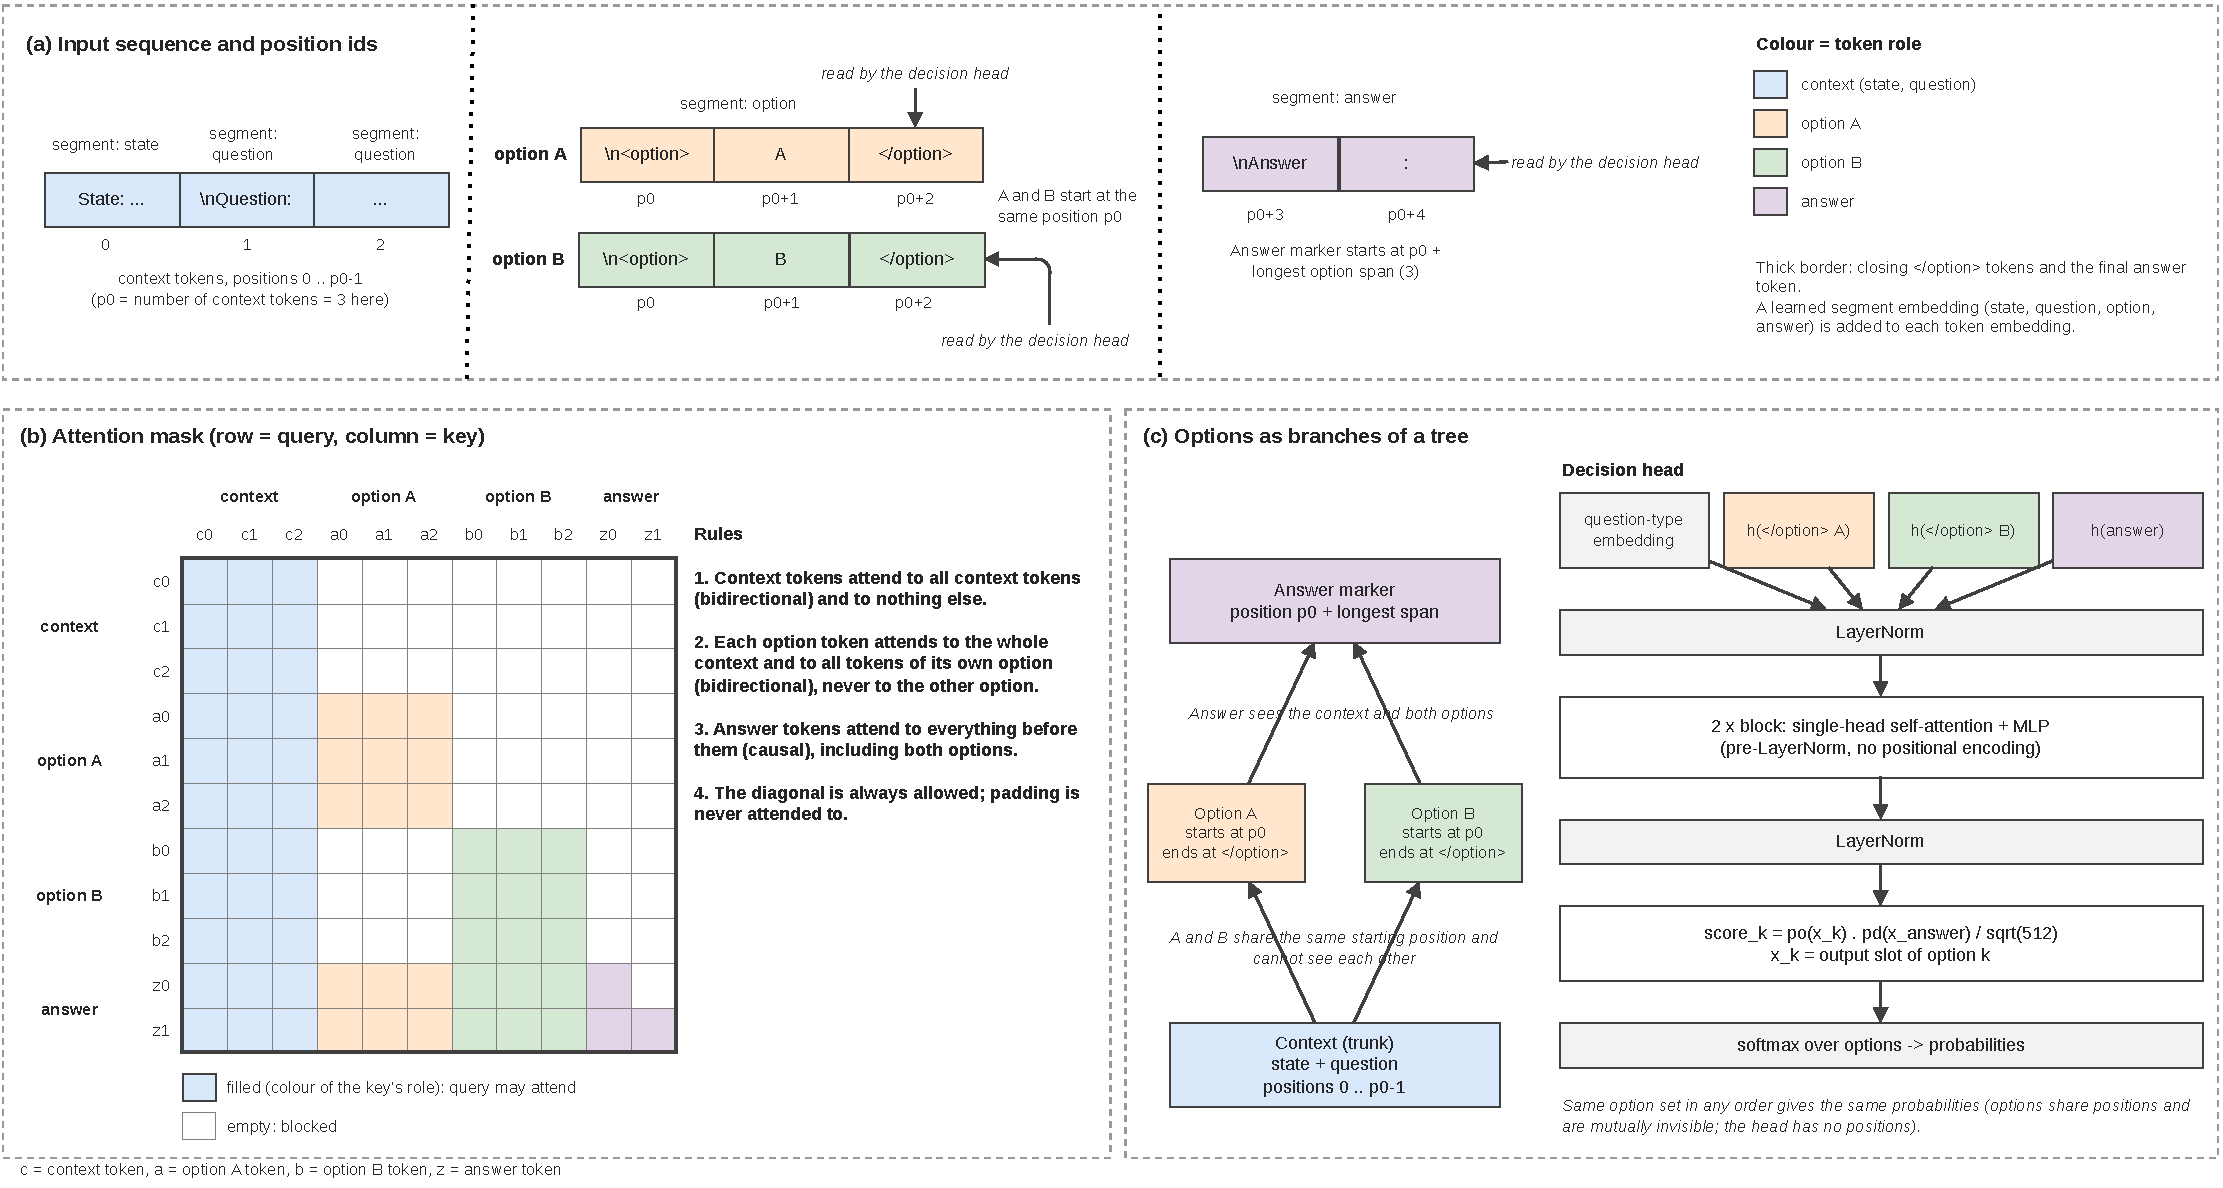
\includegraphics[width=\linewidth]{figures/prism_mask.pdf}
\caption{Input layout and attention mask for one question with two options. Context tokens attend bidirectionally; each option attends to the context and to its own tokens but not to the other option; the answer marker attends to the context and both options. Options share a start position, so they form branches of a tree. The decision head reads the closing token of each option and the answer marker.}
\label{fig:mask}
\end{figure}

\section{Streaming Inference Engine}

The engine keeps one decoder layer on the device and overlaps the disk read of the next layer with the computation of the current one (Figure~\ref{fig:engine}). The backbone is split across 33 safetensors files (one embedding file and 32 decoder-layer files), and each MoE layer is 3.35\,GB. A layer is staged in a pinned host buffer by 8 reader threads with 64\,MB reads, copied to the integrated GPU and released after use.

This schedule works because a decision model has no decode loop. A generative model visits every layer once per generated token, so streaming would pay the read cost repeatedly. Prism produces all option probabilities in one pass, so every layer is read once per batch and the read serves every question in the batch. The SSD delivers 1.2148\,GB/s with 8 threads and 64\,MB blocks, so one pass over 104,068,783,616 layer bytes has a floor of 77.2\,s. Most of the time beyond that floor is computation, not I/O.

FP8 weights are dequantised with a 256-entry lookup table that gives the same values as a native BF16 cast and reads faster (Appendix~\ref{app:details}). Routed experts are dequantised one at a time after the router has selected them, which keeps the peak device allocation small. Attention applies the Prism mask to chunked scores, which bounds the attention matrix without changing the result. The MoE block runs one grouped matrix multiply per non-empty expert, then the shared expert, and accumulates routed outputs in FP32 before a single cast to BF16. The decision head and final RMSNorm run on the CPU in FP32, matching the reference precision.

The integrated GPU has no FP8 matrix multiply, so activations are quantised to the E4M3 grid only in emulation mode. After an out-of-memory error the Intel driver did not return the device to a usable state, so all GPU runs use a fresh process and the engine checks free memory before allocating a layer.

\begin{figure}[!htbp]
\centering
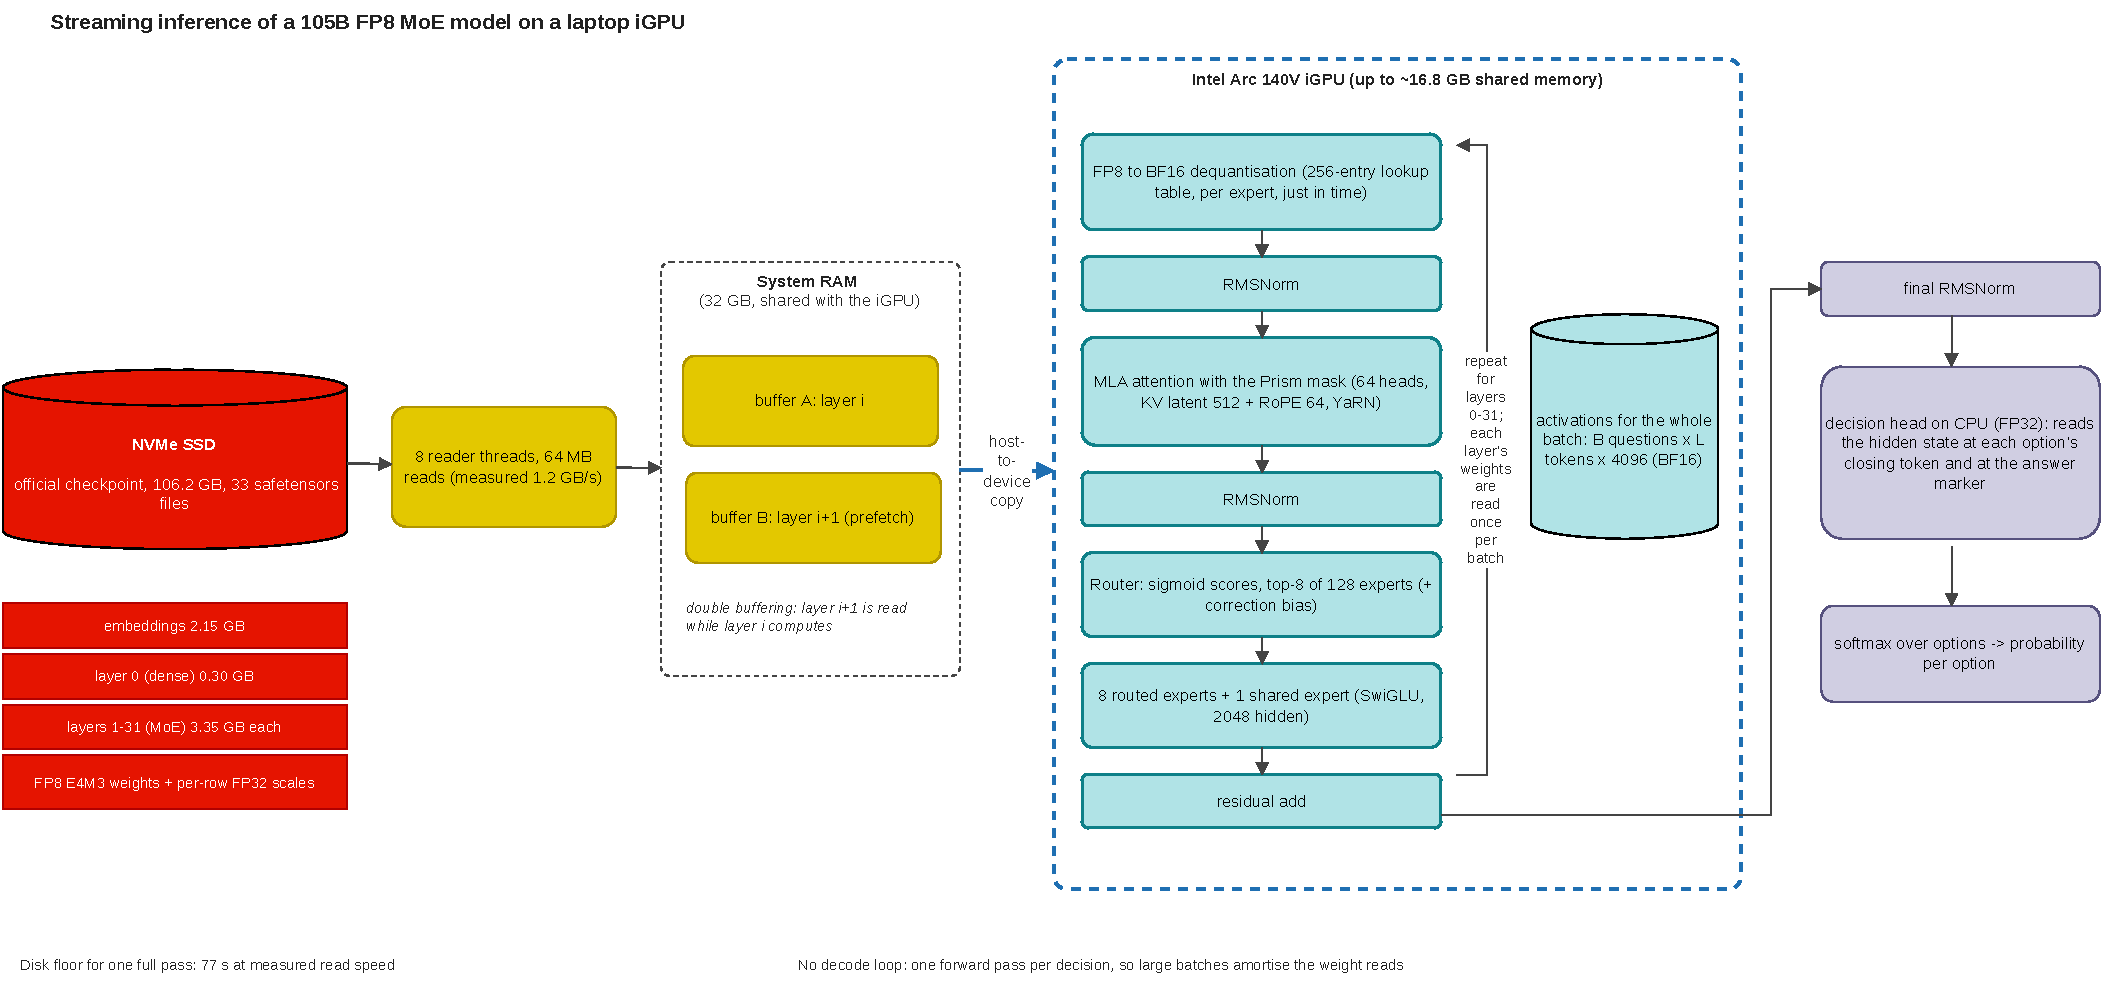
\includegraphics[width=\linewidth]{figures/engine_pipeline.pdf}
\caption{Data path of the streaming engine. The 106.2\,GB weight set is read from the NVMe SSD by 8 threads in 64\,MB blocks, with a measured read speed of 1.2148\,GB/s. One decoder layer is resident on the integrated GPU; the next layer is prefetched into a second host buffer while the current layer computes. Routed experts are dequantised from FP8 to BF16 just in time, and the final norm and decision head run on the CPU in FP32.}
\label{fig:engine}
\end{figure}

\section{Verification}

The engine matches an independent FP32 reference at the layer level, picks the same options as the model card example, and agrees with the hosted API on most questions. The model card example differs from the engine by a small probability gap that does not come from a layer-level error.

\subsection{Layer-level reference}

The FP32 path agrees with an independent FP32 CPU reference to about $10^{-7}$ relative L2 error, and the BF16 paths to about $10^{-3}$ (Table~\ref{tab:layers}, Appendix~\ref{app:verification}). The reference reads the same weights but shares no code with the engine. We run the 78-token team question of the model card example through both and compare the hidden state after layers 0 and 1; layers 2 and 3 stay at the same order of error. At layer 3 the BF16 router-weight trace crosses the stored threshold on some tokens while the hidden state remains close, which we treat as a precision limit of BF16 routing, not a functional failure. The decision head matches an independent implementation on random inputs to below $10^{-8}$.

\subsection{The model card example}

The engine selects the same options as the model card on all three questions: billing, yes and anger level 2. The maximum absolute probability difference is 0.041383, at anger level 3 (Table~\ref{tab:golden}).

\begin{table}[!htbp]
\centering
\small
\caption{The model card example in FP8-emulation mode. The largest absolute difference is 0.041383. The argmax choices match. The hosted API's maximum absolute difference from the published example is 0.080740.}
\label{tab:golden}
\begin{tabular}{lrr}
\toprule
Field & Engine & Published \\
\midrule
team: billing & 0.986213 & 0.986 \\
team: tech & 0.007307 & 0.007 \\
team: delivery & 0.006481 & 0.006 \\
urgent: yes & 0.467766 & 0.45 \\
anger: 0 & 0.035849 & 0.032 \\
anger: 1 & 0.293908 & 0.267 \\
anger: 2 & 0.520626 & 0.51 \\
anger: 3 & 0.149617 & 0.191 \\
\bottomrule
\end{tabular}
\end{table}

The gap has a history. An earlier revision measured 0.022238 on the same example, and reverting the four later edits one at a time shows that the change comes from FP32 accumulation of the routed experts, not from a loss of layer-level accuracy (Appendix~\ref{app:verification}). The exact earlier combination is not preserved, so we report it as history.

The hosted API is farther from the published probabilities than the engine, so the gap is not evidence that the engine is wrong. The layer-level comparison is the stronger check.

\subsection{Invariance and API parity}

The full model agrees with the hosted API on 93\% of the 1,200 questions that are present in every run (Table~\ref{tab:api}). Mean KL is 0.05 and accuracy is 82\% for both systems. A 50-repeat noise floor of the API has 100\% argmax agreement and mean KL 0.0003, so the gap to the full model is well above API noise. The pruned variants agree with the API far less.

The earlier revision passed four invariance checks (option order, determinism, batch composition and padding), with differences below 0.001 and determinism exact. The current engine uses the same encoder, mask and head, but we did not repeat the full sweep on it.

\begin{table}[!htbp]
\centering
\small
\caption{Parity with the hosted Sarvam Prism API on 1,200 questions. The reference is the API. KL is $\mathrm{KL}(\text{API}\,\|\,\text{system})$; the delta is system accuracy minus API accuracy in percentage points.}
\label{tab:api}
\begin{tabular}{lrrrrr}
\toprule
System & Agreement & Mean KL & Mean TV & API acc. & Delta (pp) \\
\midrule
Full & 0.9267 & 0.0474 & 0.0654 & 0.8175 & +0.17 \\
$N=32$ general & 0.7775 & 0.2773 & 0.1907 & 0.8175 & $-10.83$ \\
$N=16$ general & 0.6608 & 0.4937 & 0.2877 & 0.8175 & $-18.67$ \\
$N=32$ geometry & 0.6508 & 0.5388 & 0.3027 & 0.8175 & $-20.17$ \\
\bottomrule
\end{tabular}
\end{table}

\section{Performance}
\label{sec:perf}

Batch size is the main control: on the full model, throughput rises from 2.98 tokens per second at batch 3 to 32.02 at batch 64 (Table~\ref{tab:perf}, Figure~\ref{fig:f4}). All measurements use the same laptop: an Intel Core Ultra CPU, 32\,GB of RAM, an Intel Arc 140V iGPU with 16\,GB of shared memory and an NVMe SSD. The full model reads 104,068,783,616 bytes per pass.

\begin{table}[!htbp]
\centering
\small
\caption{Throughput on the tested laptop. The full model uses the disk-streaming mode on the integrated GPU; the pruned variants use the same mode. The CPU row uses RAM-resident weights.}
\label{tab:perf}
\begin{tabular}{llrrrr}
\toprule
Configuration & Device & Batch & Tokens & Total (s) & Tokens/s \\
\midrule
Full model & iGPU, disk & 3 & 402 & 134.8 & 2.98 \\
Full model & iGPU, disk & 16 & 2,162 & 146.3 & 14.78 \\
Full model & iGPU, disk & 64 & 8,662 & 270.5 & 32.02 \\
$N=32$ & iGPU, disk & 1 & 136 & 33.5 & 4.06 \\
$N=32$ & iGPU, disk & 16 & 2,230 & 45.2 & 49.33 \\
$N=32$ & iGPU, disk & 64 & 8,918 & 98.6 & 90.48 \\
$N=16$ & iGPU, disk & 1 & 136 & 21.3 & 6.39 \\
$N=16$ & iGPU, disk & 16 & 2,230 & 26.2 & 85.09 \\
$N=16$ & iGPU, disk & 64 & 8,918 & 79.7 & 111.89 \\
$N=16$ & CPU, RAM & 3 & 419 & 63.2 & 6.63 \\
\bottomrule
\end{tabular}
\end{table}

The pruned models scale further because their weights are smaller: $N=16$ reaches 111.89 tokens per second at batch 64. The full model is compute-bound at the largest batch, with 0.92 effective TFLOPS against a BF16 matmul peak of 12.86, so further disk tuning alone cannot make it much faster. Figure~\ref{fig:f5} shows that the 77.2\,s disk floor is under a third of the 270.5\,s total at batch 64, so larger batches raise tokens per second and also latency per batch. The three-question example takes 210.8\,s in FP8-emulation mode and 151.0\,s in BF16. The CPU-only $N=16$ run (6.63 tokens per second at batch 3) is a fallback, not a throughput competitor.

\begin{figure}[!htbp]
\centering
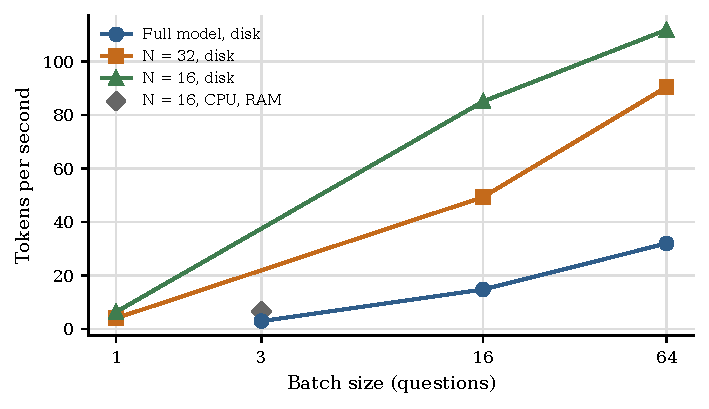
\includegraphics[width=\linewidth]{figures/f4_throughput.pdf}
\caption{Tokens per second against batch size for the full model and the two pruned variants on the integrated GPU, plus the CPU-only $N=16$ point. The horizontal axis is logarithmic in batch size.}
\label{fig:f4}
\end{figure}

\begin{figure}[!htbp]
\centering
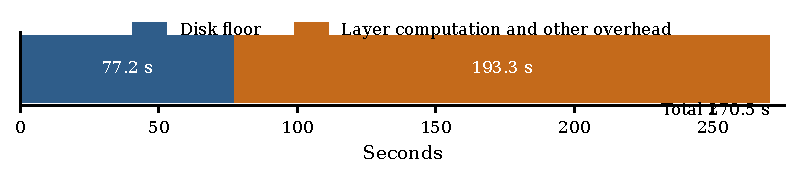
\includegraphics[width=\linewidth]{figures/f5_time_breakdown.pdf}
\caption{Time of one full-model pass at batch size 64 against the measured disk floor. The orange segment includes layer computation, host-to-device copies and other overhead.}
\label{fig:f5}
\end{figure}

\section{Expert Pruning}

Keeping 32 of 128 experts preserves classification-style decisions but not knowledge or low-resource-language decisions, and the calibration domain matters more than the ranking rule.

\subsection{Method}

The routed experts hold almost all of the weight bytes (Appendix~\ref{app:inventory}). We keep the first $N$ experts of every MoE layer under a ranking computed from a calibration pass, and rewrite the router and expert tensors so that the pruned model is a valid weight set of the same architecture with 128 replaced by $N$. Layer 0 is dense and is copied unchanged. The kept sets are nested ($N=8$ inside $N=16$ inside $N=32$), so sizes differ only in how many experts are kept.

During calibration we accumulate, for every token routed to expert $j$, the router weight $g_j(t)$ and the norm $\|f_j(t)\|$ of the expert output. The saliency sum is $S_j=\sum_t g_j(t)\|f_j(t)\|$. The REAP rule ranks by $S_j/c_j$, the mean saliency per activation, where $c_j$ is the number of tokens routed to the expert \citep{lasby2026reap}. The TOTAL rule ranks by $S_j/T$, the saliency divided by the number of tokens in the layer. TOTAL favours experts that are used often and strongly; REAP favours experts that are strong when they are used.

We use two calibration sets. The general set is 500 questions drawn from the same eleven public datasets as the test set, interleaved across datasets and languages (82,555 tokens). The narrow set is 96 synthetic geometry questions (18,760 tokens), a stress test far from the general distribution, not a claim that geometry is the target application. The two calibrations keep different experts: the mean kept-set Jaccard overlap is 0.32 at $N=32$ and 0.26 at $N=16$.

The pruned weight sets pass three checks: tensor shapes and sorted, unique, in-range ids; file sizes within a relative error of $8.43\times10^{-6}$ of the size arithmetic; and a bitwise-identical hidden state after layer 1 when layers 0 and 1 are rewritten with $N=128$ and $N=16$.

\begin{figure}[!htbp]
\centering
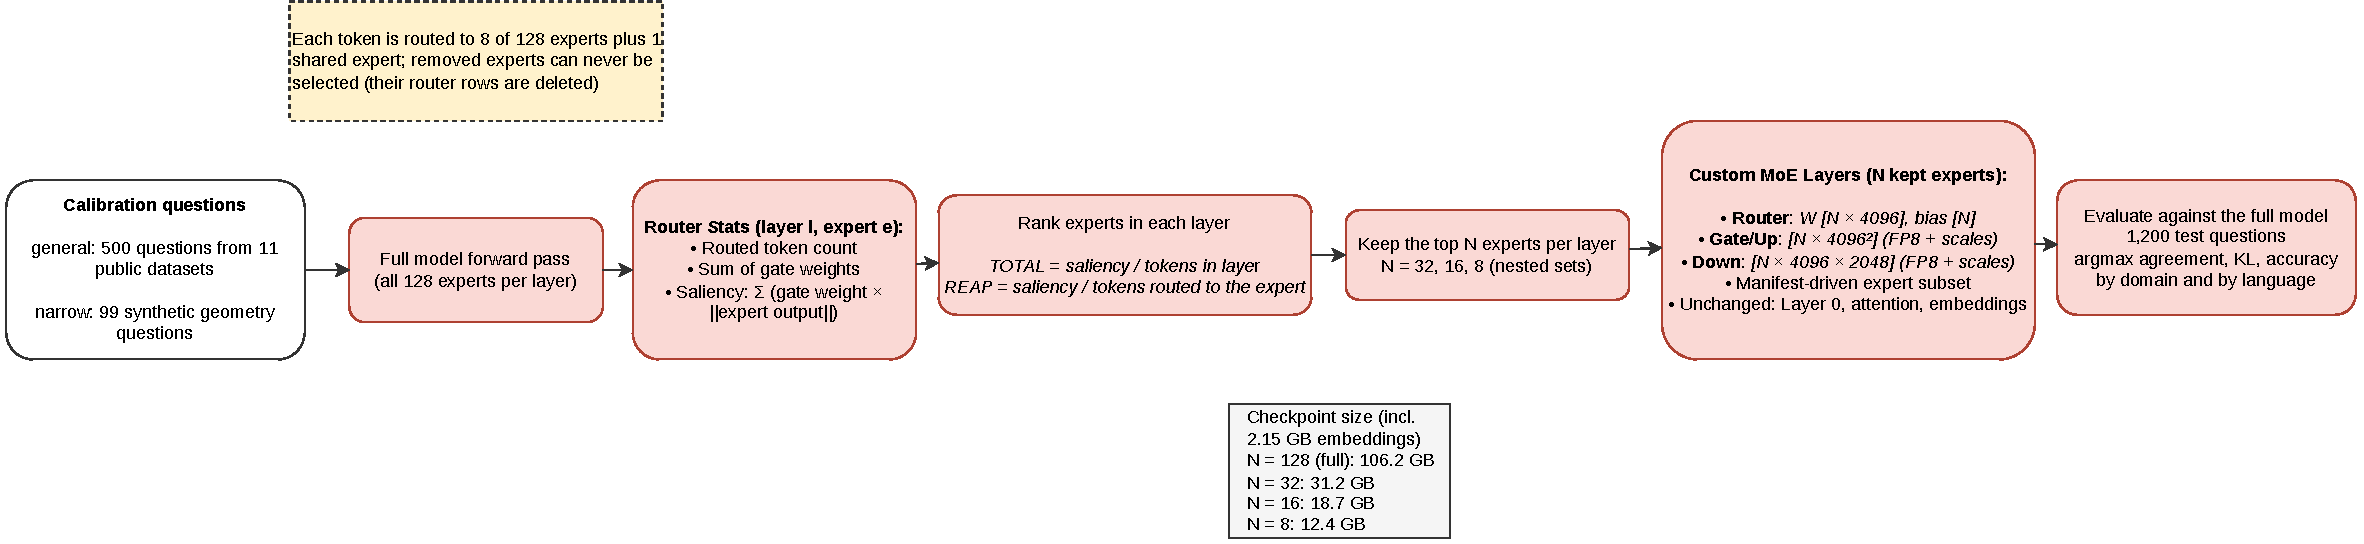
\includegraphics[width=\linewidth]{figures/pruning_pipeline.pdf}
\caption{Expert pruning pipeline. A calibration pass collects router and expert-output statistics for every MoE layer. Experts are ranked by TOTAL or REAP saliency, the top $N$ are kept in each layer, and the router and expert tensors are rewritten. The pruned weight set is compared with the full model on the test questions.}
\label{fig:pruning}
\end{figure}

\subsection{Fidelity}

Fidelity falls steadily as experts are removed, and the loss is concentrated in a few task types. The reference is the full BF16 engine with identical batching. We report argmax agreement, mean KL divergence $\mathrm{KL}(\text{full}\,\|\,\text{variant})$, mean total variation and accuracy on the labelled test set of 1,200 questions in nine domains and five languages (Table~\ref{tab:fidelity}, Figure~\ref{fig:f1}). Keeping 32 experts gives 78\% agreement and an accuracy drop of 11 points; keeping 16 gives 66\% and a drop of 19 points. REAP at $N=16$ is worse than TOTAL (63\% agreement against 66\%), and $N=8$ reaches 49\% agreement.

\begin{table}[!htbp]
\centering
\small
\caption{Fidelity of pruned variants against the full model on 1,200 test questions. Agreement is the fraction of identical argmax choices; KL is $\mathrm{KL}(\text{full}\,\|\,\text{variant})$; TV is total variation. The 95\% interval is for agreement. Accuracy is on the labelled test set.}
\label{tab:fidelity}
\begin{tabular}{lrrrrrrr}
\toprule
Variant & $N$ & Agreement & 95\% CI & Mean KL & Mean TV & Acc.\ full & Acc.\ var. \\
\midrule
N32\_general & 32 & 0.7750 & 0.7505--0.7977 & 0.2866 & 0.1949 & 0.8192 & 0.7092 \\
N16\_general & 16 & 0.6633 & 0.6361--0.6895 & 0.5148 & 0.2963 & 0.8192 & 0.6308 \\
N32\_total   & 32 & 0.6508 & 0.6234--0.6773 & 0.5626 & 0.3112 & 0.8192 & 0.6158 \\
N16\_total   & 16 & 0.5742 & 0.5460--0.6019 & 0.7535 & 0.4091 & 0.8192 & 0.5500 \\
N16\_reap    & 16 & 0.6342 & 0.6065--0.6610 & 0.5960 & 0.3494 & 0.8192 & 0.5925 \\
N8\_total    & 8  & 0.4925 & 0.4643--0.5208 & 0.8967 & 0.4823 & 0.8192 & 0.4733 \\
\bottomrule
\end{tabular}
\end{table}

\begin{figure}[!htbp]
\centering
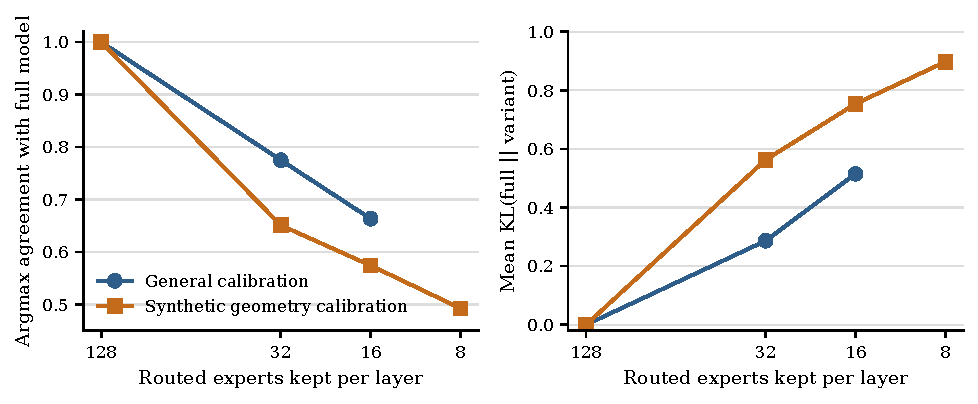
\includegraphics[width=\linewidth]{figures/f1_agreement_kl.pdf}
\caption{Agreement and KL against the full model as routed experts are removed. The general-calibration curve has no $N=8$ point because that variant was not built; the synthetic-geometry curve includes $N=8$. The full model is the identity reference at $N=128$.}
\label{fig:f1}
\end{figure}

The average hides the main result. Figure~\ref{fig:f2} splits the general-calibrated variants by domain: at $N=32$, NLI (98\%), sentiment (99\%) and intent routing (90\%) stay close to the full model, while knowledge multiple choice falls to 41\% agreement and loses 40 accuracy points. At $N=16$ knowledge multiple choice falls further, to 31\%.

\begin{figure}[!htbp]
\centering
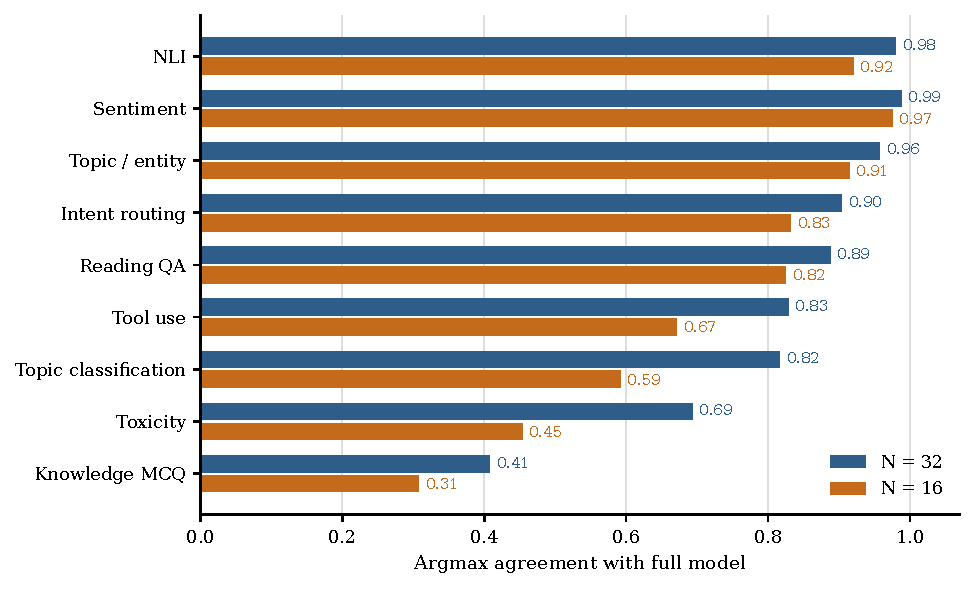
\includegraphics[width=\linewidth]{figures/f2_domain_agreement.pdf}
\caption{Argmax agreement by domain at $N=32$ and $N=16$ for the general-calibrated variants. The tasks are ordered by $N=32$ agreement.}
\label{fig:f2}
\end{figure}

Languages split the same way (Figure~\ref{fig:f3}). At $N=32$, Hindi, Bengali and Telugu agree on 63\%, 64\% and 58\% of questions, against 82\% for English and 81\% for Tamil, and their accuracy drops are 17 to 25 points against 8 for English. The general calibration set is 71\% English, so the low-resource languages lose experts that it rarely selects.

\begin{figure}[!htbp]
\centering
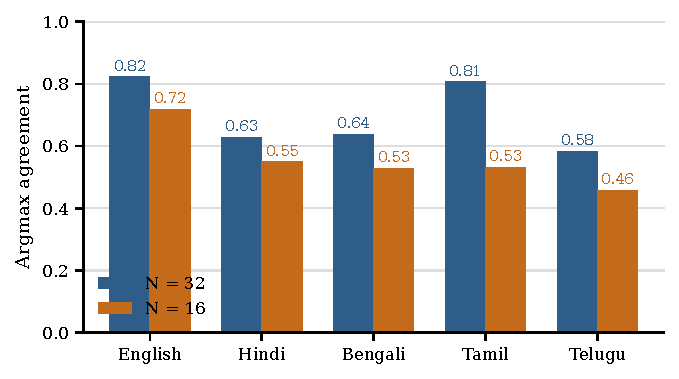
\includegraphics[width=\linewidth]{figures/f3_language_agreement.pdf}
\caption{Argmax agreement by language at $N=32$ and $N=16$ for the general-calibrated variants.}
\label{fig:f3}
\end{figure}

\subsection{Calibration and ranking}

The calibration domain decides which experts survive, and it matters more than the ranking rule. General calibration is better on the general test set at both sizes, the order reverses on the 63 held-out geometry questions, and both contrasts are larger than the TOTAL-versus-REAP contrast at either size (Table~\ref{tab:cross}). The calibration distribution, not the ranking rule, is the first decision when pruning this model.

\begin{table}[!htbp]
\centering
\small
\caption{Cross-evaluation of the calibration domains. Agreement with the full model on the general test set (1,200 questions) and on 63 held-out geometry questions. Geometry KL is $\mathrm{KL}(\text{full}\,\|\,\text{variant})$ on the geometry questions. A dash means the value was not measured.}
\label{tab:cross}
\begin{tabular}{lrrrr}
\toprule
Calibration & $N$ & General test & Geometry test & Geometry KL \\
\midrule
General & 32 & 0.7750 & 0.6984 & 0.5779 \\
General & 16 & 0.6633 & 0.4762 & -- \\
Geometry & 32 & 0.6508 & 0.9683 & 0.0261 \\
Geometry & 16 & 0.5742 & -- & -- \\
\bottomrule
\end{tabular}
\end{table}

\subsection{Layer skipping}
Skipping whole decoder layers costs much more fidelity than expert pruning at comparable size. On the 63 held-out geometry questions, skipping two layers lowers the agreement of the 32-expert geometry-calibrated model from 97\% to 71\%; we do not claim a general rule from 63 questions (Appendix~\ref{app:details}).

\section{Related Work}

\paragraph{Expert pruning and merging.}
Sparse MoE layers activate a few experts per token \citep{shazeer2017outrageously,fedus2022switch,jiang2024mixtral}, but the full parameter count still dominates memory, so several methods remove experts after training. Lu et al.\ prune by reconstruction loss on a calibration set and add dynamic expert skipping \citep{lu2024experts}. REAP ranks experts by the router-weighted norm of their output and argues that pruning keeps routing control that merging loses \citep{lasby2026reap}. MoE-Pruner scores weights with router weights and input activations \citep{xie2024moepruner}. We use similar router statistics but ask which decision tasks survive and how much the calibration distribution matters.

\paragraph{Weight offloading and layer streaming.}
DeepSpeed-Inference combines GPU, CPU and NVMe memory to serve models larger than GPU memory \citep{aminabadi2022deepspeed}, and FlexGen searches tensor placement and batch schedules on one commodity GPU \citep{sheng2023flexgen}. PowerInfer keeps hot neurons on the GPU and cold ones on the CPU \citep{song2024powerinfer}, and Eliseev and Mazur cache and prefetch experts during generation \citep{eliseev2023offloading}. All of these assume autoregressive decoding. A decision model needs one forward pass, so streaming reduces to a single sequential read of the weights.

\paragraph{Classification heads and decision models.}
BERT-style encoders are adapted to classification with a small head on a pooled representation \citep{devlin2019bert}, and Sentence-BERT and SetFit pair sentence representations with a light classifier \citep{reimers2019sentence,tunstall2022setfit}. Prism scores options jointly: option spans share a context, cannot see each other and meet only at the answer marker \citep{sarvam2026prism}. Our pruning results therefore describe a 105B joint scorer, not classification heads in general.

\section{Limitations}

The measurements come from one laptop with one integrated GPU and one SSD, and we did not test NVIDIA hardware, a discrete GPU or a different disk. The FP8 path is emulated in BF16, so native FP8 hardware would change both speed and numerics. The engine is slow in absolute terms. The 63 held-out geometry questions are a small evaluation set, so the layer-skip comparison is a measurement, not a general rule. We did not test other Indian languages, long contexts, code, security prompts or top-$k$ values other than 8. The API parity uses recorded responses and the hosted service may change. The invariance sweep was run on the earlier revision.

The model card example is not reproduced exactly: the engine matches the model's decisions but not every published probability. TOTAL and REAP are first-order saliency heuristics, and the low overlap between the two calibrations shows that the ranking is sensitive to the calibration distribution. A production system would need a calibration set that covers its languages and decision types, with a held-out check for each.

\section{Conclusion}

A 105B FP8 decision model runs correctly on a laptop integrated GPU when it is streamed one decoder layer at a time. The engine agrees with an independent FP32 reference, reproduces the model card's choices and tracks the hosted API closely. It is slow in absolute terms, and the disk floor is a minor part of the cost at large batches.

Expert pruning gives a boundary rather than a single number. Keeping a quarter of the experts preserves classification-style decisions and loses knowledge and low-resource-language decisions, and the calibration domain matters more than the ranking rule. A pruned decision model should be calibrated for the decisions and languages it will serve. The engine and result files are public. A native FP8 implementation and a mixed calibration set with per-language held-out checks are the next steps.

\appendix
\section{Verification Details}
\label{app:verification}

\subsection{Layer-level numbers}

Table~\ref{tab:layers} reports the hidden-state comparison after layers 0 and 1. Extending the check to layers 2 and 3 gives relative L2 errors of $4.79\times10^{-3}$ and $5.51\times10^{-3}$ in BF16 and $6.35\times10^{-3}$ and $8.51\times10^{-3}$ in FP8 emulation. At layer 3 the BF16 router-weight trace has minimum cosine 0.778 and relative L2 0.0905. The decision head differs from an independent implementation by at most $4.48\times10^{-9}$.

\begin{table}[!htbp]
\centering
\small
\caption{Hidden-state comparison against the FP32 CPU reference after layers 0 and 1. The sequence is the 78-token team question. Cosine is the minimum over tokens; relative L2 is over the whole hidden state.}
\label{tab:layers}
\begin{tabular}{lrrrr}
\toprule
Mode & L0 cos & L0 rel. L2 & L1 cos & L1 rel. L2 \\
\midrule
FP32 & 0.9999998 & $3.40\times10^{-7}$ & 0.9999996 & $3.92\times10^{-7}$ \\
BF16 & 0.9999920 & $2.92\times10^{-3}$ & 0.9999868 & $3.78\times10^{-3}$ \\
BF16 + FP8 emulation & 0.9999858 & $3.40\times10^{-3}$ & 0.9999689 & $4.64\times10^{-3}$ \\
\bottomrule
\end{tabular}
\end{table}

\subsection{History of the gap and invariance checks}

An earlier revision measured a maximum gap of 0.022238 on the model card example. The preserved code was edited after the earlier measurement, so it is numerically equivalent to the current engine. We reverted the four edits one at a time in a scratch copy. Reverting the FP32 accumulation in the MoE to BF16 moves the FP8-emulation gap to 0.111615, the largest change of any revert. Reverting the attention scale to the value without the YaRN multiplier gives 0.070594 in FP8 emulation and 0.050096 in BF16. The activation-scale path changes the result by $9.9\times10^{-6}$ and the RoPE layout is numerically neutral. The larger gap is a change in accumulation order, not a loss of layer-level accuracy. The exact 0.022238 combination is not preserved.

The earlier invariance checks gave maximum absolute differences of 0.000761 for option order, 0.0 for determinism, 0.000506 for batch composition and 0.0000435 for padding. In the 50-repeat API noise floor, mean absolute difference is 0.001531, mean KL 0.000324 and mean total variation 0.003252.

\section{Dequantiser Speed and Layer Skipping}
\label{app:details}

The E4M3 lookup table has 254 finite codes, a largest finite value of 448.0 and a smallest positive value of 0.001953125. In the measured reader loop the lookup table reaches 0.8458\,GB/s, the native BF16 cast 0.5063\,GB/s and a bit-manipulation path 0.1041\,GB/s.

On the 63 held-out geometry questions, the unskipped $N=32$ geometry-calibrated model reaches agreement 0.9683, KL 0.0261 and accuracy 0.7302 at 70.1 tokens per second. Skipping layers 20 and 28 gives agreement 0.7143 and KL 0.4141; skipping layers 20, 25, 28 and 29 gives agreement 0.7302 and KL 0.4656. The four-layer skip is not worse than the two-layer skip on this small set. Skipping two layers drops agreement by 0.253968.

\section{Tensor Inventory and Reproduction}
\label{app:inventory}

\subsection{Inventory and size arithmetic}

The weight set contains 732 backbone tensors in 33 files: one embedding file and 32 decoder-layer files; the decision head is a separate file. The backbone totals 106,216,275,456 bytes; the decision head adds 117,837,824 bytes. Routed experts account for 99,988,013,056 of those bytes, attention for 3,032,588,288, embeddings for 2,147,483,648 and shared experts for 781,156,352; the router, dense MLP and norms make up the rest.

Let $b_e=25{,}198{,}592$ be the bytes of one routed expert, $b_r=16{,}388$ of one router row, $b_s=25{,}198{,}592$ of the shared expert and $b_a=94{,}784{,}768$ of the attention block. One MoE layer with $N$ kept experts has $B_{\text{layer}}(N) = N(b_e+b_r)+b_s+b_a$ bytes, and the 32-layer backbone has $B_{\text{total}}(N) = 31\,B_{\text{layer}}(N) + B_{\text{layer 0}}$ with $B_{\text{layer 0}}=296{,}258{,}816$. Table~\ref{tab:sizes} evaluates this for the sizes used in the study.

\begin{table}[!htbp]
\centering
\small
\caption{Weight-set size for different expert counts. The total column is the 32-layer backbone; the embedding column adds the 2,147,483,648-byte embedding file.}
\label{tab:sizes}
\begin{tabular}{rrrrr}
\toprule
$N$ & Layer bytes & 31 layers & Total bytes & With embedding (GB) \\
\midrule
128 & 3,347,500,800 & 103,772,524,800 & 104,068,783,616 & 106.216 \\
32 & 926,862,720 & 28,732,744,320 & 29,029,003,136 & 31.176 \\
16 & 523,423,040 & 16,226,114,240 & 16,522,373,056 & 18.670 \\
8 & 321,703,200 & 9,972,799,200 & 10,269,058,016 & 12.417 \\
\bottomrule
\end{tabular}
\end{table}

\subsection{Environment and reproduction}

The measurements use Python 3.11, torch 2.9.1+xpu and driver 1.6.34541 on the laptop described in Section~\ref{sec:perf}. The measured BF16 matmul throughput is 12.860 TFLOPS at $4096^3$, and the host-to-device copy rate is 0.7924\,GB/s.

The public repository contains the engine, the result files and the scripts that produced them. The main commands, run from the repository root, are:
{\footnotesize
\begin{verbatim}
python scripts/inventory.py --weights weights
python scripts/verify_layers.py --weights weights
python scripts/golden.py --weights weights
python scripts/perf.py --weights weights --out results
python scripts/build_pruned.py --weights weights --ranking total --n 32,16 --out results
python scripts/run_eval.py --weights weights --variant N32_general --split test --out results
python scripts/api_parity.py
\end{verbatim}}
The README has the full command list. The evaluation set is built from public datasets with their licences recorded in \texttt{results/eval/datasets.json}; question text is not redistributed.

\bibliographystyle{plainnat}
\begingroup
\scriptsize
\setlength{\bibsep}{0pt}
\bibliography{refs}
\endgroup

\end{document}
